\chapter{Frontend}

Bevor das Frontend in seiner endgültigen Form entworfen und ausgearbeitet wurde, ist die grundsätzliche Eignung und Anwendbarkeit der geplanten Architektur-Ideen in einem Prototyp getestet worden. Der grundsätzliche Aufbau konnte dann bei der Implementation der finalen Version beibehalten werden, zusätzlich musste aber noch die Anbindung an den Erkennungs-Dienst vorgenommen und ein \emph{InputMethodService} musste implementiert werden.

\section{Analyse}

Zuerst wollen wir nun kurz der generelle Funktionsweise eines solchen Dienstes betrachten, bevor die erarbeitete Lösung erläutern wird.

\subsection{InputMethodService}

Das Android Betriebssystem erlaubt es, dass Applikationen von Drittanbietern die systemweit zur Eingabe von Text verwendete Applikation durch eine eigene ersetzten. Diese ``Input Method'' wird dabei ebenfalls als Hintergrund-Dienst betrieben, um eine möglichst verzögerungsfreie Texteingabe zu ermöglichen. Es liegt als nahe, einen solchen Dienst für unser Frontend zu implementieren, um es dem Benutzer zu ermöglichen, Eingaben in jegliche Textfelde handschriftlich durchzuführen. \cite{adg_ime}

Die vom Android-SDK bereitgestellte Klasse \emph{InputMethodService} muss uns dabei als Basis dienen. Sie definiert die Methoden, welche den Lebenszyklus des Dienstes und seine Interaktion mit den Eingabefeldern regeln.

\subsection{Benutzer-Schnittstelle}

Die Benutzer-Schnittstelle zur Eingabe der Zeichen soll vollständig auf die Bedienung per Touchscreen ausgelegt werden. Somit sollen keine Klicks auf Buttons den Eingabefluss des Benutzers stören.
%================================================

\section{Design}

Wie bereits festgestellt, müssen wir unsere Eingabe-Methode in Form der Klasse \emph{HandwritingIME} von der Basis-Klasse \emph{InputMethodService} ableiten. Um die grafischen Bedienelemente vom Dienst abzukoppeln definiert die Basis-Klasse Methode zur Erzeugung and Anzeige eines Input-\emph{Views} und bietet auch für diesen eine Basis-Klasse namens \emph{KeyboardView} an, von welcher wir einen eigenen \emph{View} names \emph{PadView} ableiten wollen. Für die Rückmeldung von dessen Änderungen an den Dienst wurde das Observer Design Pattern angewendet\cite[S.293-303]{designpatterns}.

\begin{figure}[h!]
   \centering
   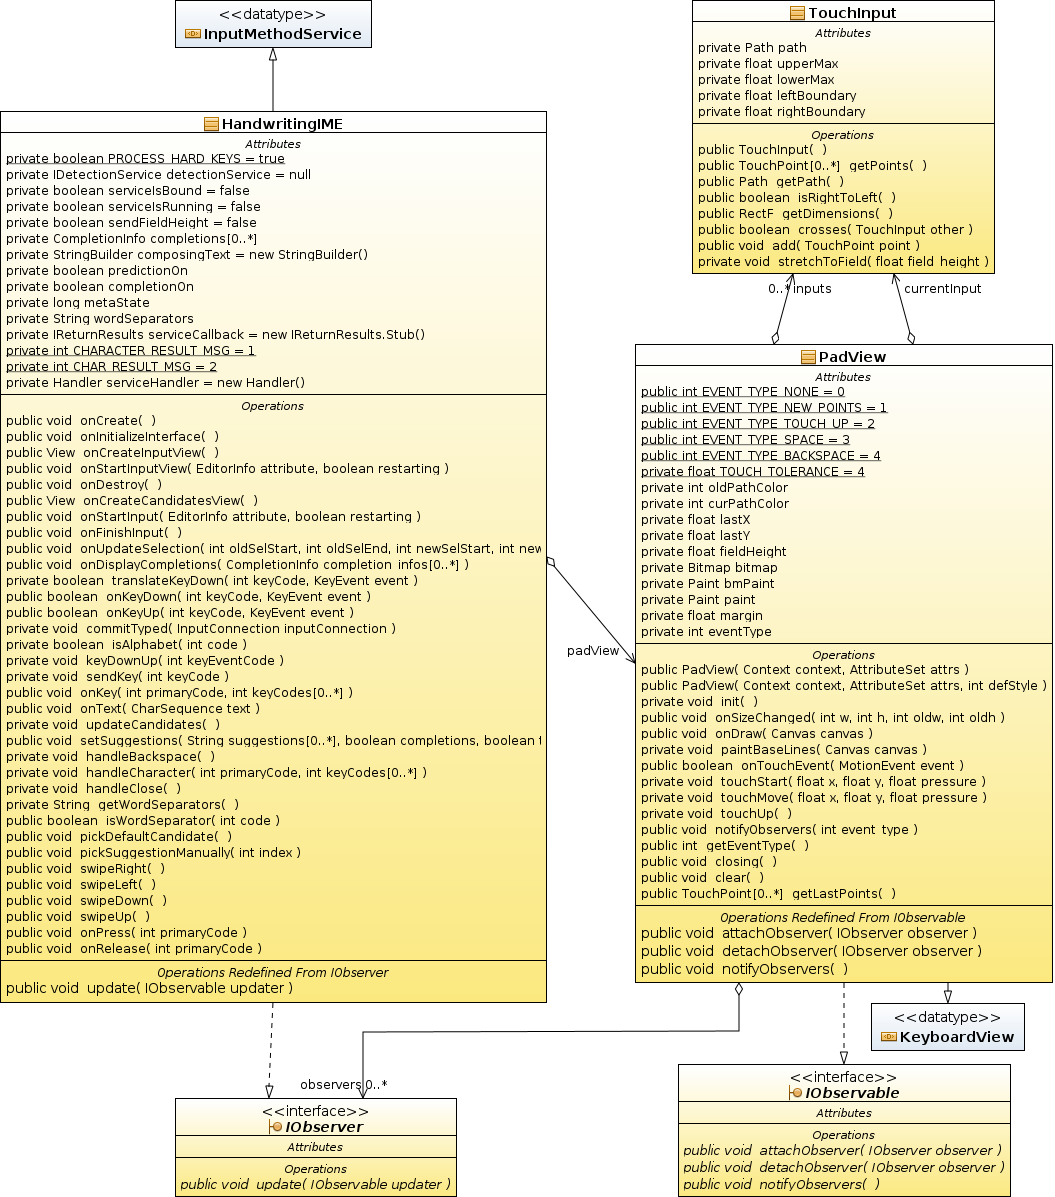
\includegraphics[width=\textwidth]{img/uml_cd_ime} 
   \caption{Klassen-Diagramm des Frontends}
   \label{fig:cd_ime}
\end{figure}

\subsection{Dienst der Eingabe-Methode}

Die von \emph{InputMethodService} abgeleitete Klasse \emph{HandwritingIME} implementiert das Interface \emph{IObserver} über Änderungen in \emph{PadView} benachrichtigt werden zu können. Ausserdem ist sie für die Kommunikation mit dem Erkennungs-Dienst zuständig und implementiert die Methoden zur Verwaltung des Lebenszyklus des Eingabe-Dienstes. Wenn der Dienst gestartet wird, soll er auch den Dienst zur Zeichen-Erkennung starten und sich an diesen binden. Diese Bindung soll erst aufgehoben werden, wenn der eigene Dienst beendet wird. Das Aufstarten von \emph{DetectionService} soll dabei in der Methode \emph{onCreate()}  erfolgen, während in \emph{onStartInputView()}, also wenn das Benutzer-Interface angezeigt wird, zu diesem gebunden werden sollt. Das Aufheben der Bindung soll in der Methode \emph{onDestroy()} erfolgen, der Erkennungs-Dienst soll aber dabei nicht explizit beendet werden um sich dessen Initialisierung bei der nächsten Verwendung zu ersparen\footnote{Wird ein \emph{Service} unter Android nicht explizit gestartet vor dem Binden, wir er nach der Aufhebung der letzten Bindung automatisch terminiert. Ansonsten läuft er unter Umständen auch ohne angebundene Clients weiter.}.

Das Erzeugen des \emph{PadViews} erfolgt in der Methode \emph{onInitializeInterface()} und das Auslesen der Eingabe-Punkte in der Methode \emph{update()} die durch das \emph{IObserver} Interface im Rahmen des Observer Patterns definiert wurde.

\subsection{Grafische Benutzeroberfläche}

Für die Annahme und Darstellung der Eingabe-Punkte ist die von \emph{KeyboardView} abgeleitete Klasse \emph{PadView} zuständig. Die Basis-Klasse würde normalerweise verwendet werden, um das Tastatur-Layout des \emph{Views} aus einer XML-Datei auszulesen und entsprechend aufzubauen. Da wir aber keine Tasten wollen können wir dies ignorieren und unsere Oberfläche selber auf den \emph{PadView} zeichnen, was in der Methode \emph{onDraw()} erfolgt.

Auf Eingaben über den TouchScreen reagiert der \emph{PadView} über die Methode \emph{onTouchEvent()}, welche uns einem \emph{Event} liefert, der neben der entsprechenden Position und dem Druck mit der die Eingabe erfolgt ist auch die Art des Ereignisses liefert. Je nachdem ob dies nun ein Aufsetzen, Verschieben oder Absetzen des Fingers ist, wird dies von einer entsprechenden Methode abgehandelt. Eine ganze solche Ereignis-Kette wird dabei in eine Instanz der Klasse \emph{TouchInput} abgespeichert, welche später auch für die Darstellung des Pfades einer solchen Eingabe zuständig ist.

Um Eingabe-Ereignisse an den Dienst der Eingabe-Methode zurück zu liefern implementiert \emph{PadView} das Interface \emph{IObservable}. Für das Observer Design Pattern wird dazu eine Liste der angehängten \emph{IObserver} verwaltet und diese werden über die Methode \emph{notifyObservers()} über Änderungen informiert. Dabei können sie durch die Methode \emph{getEventType()} die Art des Ereignisses auslesen.
%================================================

\section{Implementation}

Für die Klasse \emph{HandwritingIME} soll hier die Implementation der Handhabung von Rückmeldungen, sowohl vom Erkennungs-Dienst wie auch von der grafischen Benutzerschnittstelle betrachtet werden. Für \emph{PadView} wollen wir die Reaktion auf Touchscreen-Eingaben erläutern.

Als Grundlage für die Entwicklung des Frontend diente das Beispiel ``SoftKeyboard'', welches mit dem Android SDK mitgeliefert wird. Für das Verständnis der detaillierten Funktionsweise eines \emph{InputMethodServie} wäre es zu empfehlen, dieses zu analysieren.

\subsection{HandwritingIME}

Wie bereits erwähnt, erfolgen nach dem Starten des \emph{PadViews} in der Methode \emph{onStartInputView} dessen Rückmeldungen über die Methode \emph{update()}. Je nach dem Typ des gemeldeten Ereignisses werden entweder die neuen Eingabe-Punkte an den Erkennungs-Dienst weiter gereicht, oder es wird direkt eine entsprechende Eingabe an das derzeit aktive Eingabefeld gesendet. Dazu stellt Android die Klasse \emph{InputConnection} zur Verfügung. Die Verbindung mit dem aktiven Feld kann über der Methode \emph{getCurrentInputConnection()} erhalten werden. Über diese Schnittstelle können dann \emph{KeyEvents} erzeugt und an das Eingabefeld gesendet werden, aber auch eine direkte Manipulation des Textes um den Cursor kann vorgenommen werden.


\begin{lstlisting} [caption={Reaktion auf Eingaben in \emph{HandwritingIME}},label=ime_update]
  public void update(IObservable updater) {
    if (updater instanceof PadView) {
      if (serviceIsBound && (detectionService != null)) {
        try {
          InputConnection ic = 
            getCurrentInputConnection();
          switch (padView.getEventType()) {
            case PadView.EVENT_TYPE_NEW_POINTS :
              //...
              detectionService.addTouchPoints(
                new ArrayList<TouchPoint>(
                  padView.getLastPoints()), false);
              break;
            case PadView.EVENT_TYPE_TOUCH_UP :
              //...
              if (padView.getLastPoints() != null) {
                detectionService.addTouchPoints(
                  new ArrayList<TouchPoint>(
                    padView.getLastPoints()), true);
              } else {
                detectionService.endSample();
              } break;
            case PadView.EVENT_TYPE_SPACE :
              ic.commitText(" ", 1); break;
            case PadView.EVENT_TYPE_BACKSPACE :
              handleBackspace(); break;
          }
        } catch (RemoteException ex) {}
      }
    }
  }
\end{lstlisting}

Für die Entgegennahme der erkannten Zeichen vom Erkennungs-Dienst muss wiederum zuerst ein Stub der Rückruf-Schnittstelle (siehe Kapitel \ref{lbl_be_intrf}) implementiert werden. Diese reicht dann die erhaltenen Zeichen an einen entsprechenden Handler weiter, der diese über die aktuelle \emph{InputConnection} an das aufrufende Textfeld senden.

\begin{lstlisting} [caption={R\"{u}ckgabe der Resultate in \emph{HandwritingIME}},label=ime_results]
  private IReturnResults serviceCallback = 
    new IReturnResults.Stub() {
    public void recognisedCharacters(
      List<ch.zhaw.ba10_bsha_1.Character> characters) 
      throws RemoteException {
      serviceHandler.sendMessage(
        serviceHandler.obtainMessage(
          CHARACTER_RESULT_MSG, characters));
    }
    //...
  };
  private static final int CHARACTER_RESULT_MSG = 1;

  private Handler serviceHandler = new Handler() {
    public void handleMessage(Message msg) {
      switch (msg.what) {
        case CHARACTER_RESULT_MSG:
          ArrayList<Character> chars = 
            (ArrayList<Character>) msg.obj;
          if (chars.size() > 0) {
            InputConnection conn = 
              getCurrentInputConnection();
            StringBuffer text = new StringBuffer();
            for (Character character : chars) {
              if (!character.toString().startsWith(
                "none")) {
                text.append(
                  character.getDetectedCharacter());
              }
            }
            conn.commitText(text, 1);
          }
          break;
        //...
        default:
          super.handleMessage(msg);
      }
    }
  };
\end{lstlisting}

\subsection{PadView}

Wir wollen nun die Implementation von zwei Spezialfällen von Eingaben betrachten. Zum einen soll, wenn die neue Eingabe einen genügenden Abstand zur letzten hat, die Eingabe eines Leerzeichens an die Observer gemeldet werden. Weiter soll die Eingabe eines Backspaces gemeldet werden, wenn die neue Eingabe die jeweils letzte vollständig und von rechts nach links\footnote{Bei einem Strich von links nach rechts könnte es sich auch um die Mittellinie eines 't' oder 'f' handeln.} durchstreicht.

Dies wird im Falle des Leerzeichens beim Start einer neuen Eingabe überprüft, während die Überprüfung beim Löschen beim Absetzen erfolgt.

\begin{lstlisting} [caption={Touchscreen-Eingaben in \emph{PadView}},label=padview_touchevent]
  private void touchStart(
    float x, float y, float pressure) {
    //Rueckmelden, wenn Abstand zum letzten gross genug
    if (inputs.size() > 0) {
      RectF last = 
        inputs.get(inputs.size() - 1).getDimensions();
      if (x > (last.right + last.width())) {
        notifyObservers(EVENT_TYPE_SPACE);
      }
    }
    currentInput = new TouchInput();
    currentInput.add(new TouchPoint(x, y, pressure)); //...
  }
  private void touchUp() {
    if (inputs.size() > 0) {
      TouchInput last = inputs.get(inputs.size() - 1);
      //Testen ob neue Eingabe eine alte durchstreicht
      if (currentInput.crosses(last) 
          && currentInput.isRightToLeft()) {
        inputs.remove(last);
        notifyObservers(EVENT_TYPE_BACKSPACE);
      //Sonst Eingabe zu den fertigen fuegen 
      //und Observer benachrichtigen
      } else {
        inputs.add(currentInput);
        notifyObservers(EVENT_TYPE_TOUCH_UP);
      } currentInput = null; //...
    }
  }
\end{lstlisting}
%================================================

